\chapter{线性回归的实际形式}

\cref{cht:lr-basic}和\cref{cht:lr-extended}从基本理论出发介绍了线性回归最纯粹的形式,但是在实际应用中还有一些额外的考虑,一般需要对基本形式进行扩展。
本章介绍最常见也是最重要的两种,一种是对参数取值范围进行正则化的扩展,称为\emph{山脊回归(ridge regression)},另一种是对参数按照敏感性进行选择的扩展,称为\emph{LASSO回归(least absolute shrinkage and selection operator)}。

\section{山脊回归}
在\cref{ssec:sse-minimize}中我们把线性回归的最优参数$\Vtheta^*$定义为残差平法和最小,即
\begin{equation}
    \Vtheta^* = \argmin_{\Vtheta}\, \Ve^T\Ve。
\end{equation}
对于低次多项式这样得到的拟合函数和数据点吻合的比较好,但对于高次多相式常常出现过拟合问题。
问题的根源在于直接线性回归得到的参数$\Vtheta^*$中常常包含绝对值非常大的权重系数$w_i$。
根据拟合函数公式
\begin{equation}
    y=w_1x_1+w_2x_2+\cdots+ w_m x_m + b
\end{equation}
当权重的绝对值$|w_i|$非常大时,自变量$x_i$的微小误差在因变量$y$中会被显著放大。

为了解决过拟合问题,一个可行的思路是控制$w_i$,避免出现绝对值太大的情况。
为此我们可以在最优参数的定义中加入一个\emph{惩罚项},得到
\begin{equation}\label{eq:ridge-regression}
    \Vtheta^* = \argmin_{\Vtheta}\,\Ve^T\Ve + \lambda\Vtheta^T\Vtheta,
\end{equation}
其中参数的平方和$\Vtheta^T\Vtheta$是惩罚项,$\lambda$是权重系数。
由于惩罚项的存在,参数$\Vtheta$的绝对值有趋于$0$的趋势,$\lambda$越大趋势越明显,由此能够避免出现参数绝对值过大的情况。

\cref{eq:ridge-regression}一般称为\emph{山脊回归},要理解这个名字的由来我们需要把公式右侧的目标函数展开
\begin{align}
    \Ve^T\Ve + \lambda\Vtheta^T\Vtheta &=
    (\Vy-\MA\Vtheta)^T(\Vy-\MA\Vtheta) + \lambda\Vtheta^T\Vtheta \nonumber\\
    &=(\Vtheta^T\MA^T\MA\Vtheta+\lambda\Vtheta^T\Vtheta)-2\Vtheta^T\MA\Vy+\Vy^T\Vy\nonumber\\
    \intertext{利用单位矩阵$\MI$的性质$\Vtheta^T\Vtheta=\Vtheta^T\MI\Vtheta$}
    &=\Vtheta^T(\MA^T\MA+\lambda\MI)\Vtheta-2\Vtheta^T\MA^T\Vy+\Vy^T\Vy。
\end{align}

利用类似\cref{eq:regression-derivative}的推理方式,最优参数$\Vtheta^*$应该出现在目标函数导数的$0$点,即
\begin{equation}
    (\MA^T\MA+\lambda\MI)\Vtheta^*=\MA^T\Vy。
\end{equation}
通过与原始的线性回归公式$\MA^T\MA\Vtheta^*=\MA^T\Vy$比较,我们可以看到两个求解最优参数的方程基本相同,唯一的区别是矩阵从$\AA^T\MA$变成了$\MA^T\MA+\lambda\MI$。
如果我们把矩阵想象成等高线地形图,矩阵中的数字代表网格点上的高度,那么单位矩阵对角线为$1$其余位置为$0$的形状就像一条山脊(ridge);在$\MA^T\MA$基础上加$\lambda\MI$可以形象的想象成在地形中间抬起一条高度为$\lambda$的山脊,山脊回归由此得名。

\begin{figure*}
    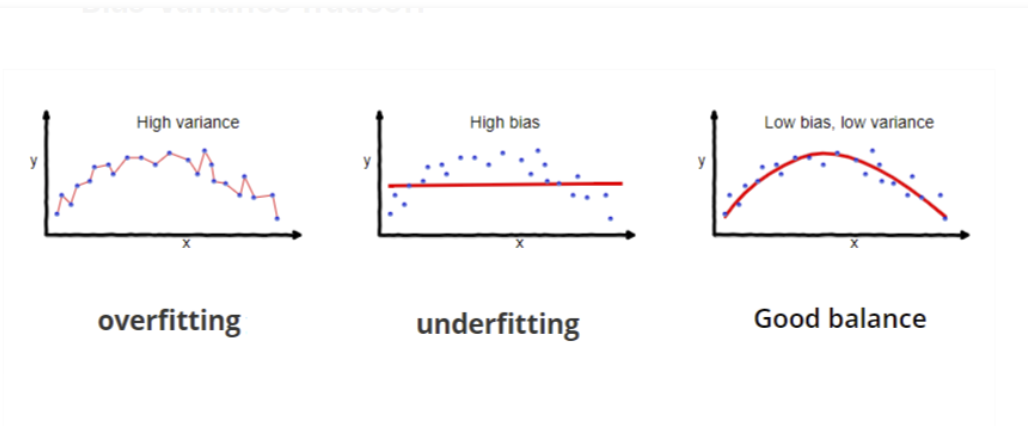
\includegraphics[width=\linewidth]{images/under_over_fit.png}
    \caption{$\lambda$值决定拟合函数是过拟合、欠拟合还是适度拟合。}
    \label{fig:under_over_fit}
\end{figure*}

要直观的理解山脊回归的功能可以先考虑$\lambda$的两种极端情况$\lambda=0$和$\lambda=\infty$。
当$\lambda=0$时$\lambda\MI=0$,山脊回归等价于基本的线性回归,此时拟合函数在$y$方向上剧烈震荡。
当$\lambda=\infty$时方程左侧的$\MA^T\MA$可以忽略不计,$\Vtheta^*=\MA^T\Vy/\infty=0$,即所有参数都是$0$,此时拟合函数是一条直线。
实际应用中我们的目标是适当选取$\lambda$值,让拟合函数形状介于两种极端之间,既保持光滑,又符合数据总体趋势,如\cref{fig:under_over_fit}所示。

\section{LASSO回归}

在实际使用线性回归,尤其是高维度的多元线性回归时,通常面临\emph{属性选择}问题。
例如我们用线性回归根据出行者的社会经济背景$\Vx$预测他的日平均出行次数$y$。
这里$y$是一个标量,而$\Vx$是一个高维向量,包含了出行者所有社会经济\emph{属性},例如年龄、性别、教育水平、收入、职业等等。

这里我们假设一共有$100$种不同的属性,但其中只有少数对出行次数有显著影响,问题是如何识别出这些属性。一种识别方法是对数据进行线性回归,得到参数向量$\Vtheta^*$,然后根据参数确定取舍。
对于第$i$个属性,如果对应的权重参数$w_i=0$,显然该属性对出行量没有影响,可以舍弃;反之有影响,保留。这种方法要求参数向量$\Vtheta^*$最好具有\emph{稀疏性},即多数元素为$0$,少数元素不为$0$。
基础的线性回归并不能保证这一点,参数向量中会出现大量绝对值很小但又不完全为$0$的元素,让属性选择无效。

LASSO回归就是能够保证参数稀疏性的回归方法。它的改进方法和山脊回归类似,也是对优化目标函数添加惩罚项,有
\begin{equation}\label{eq:lasso-regression}
    \Vtheta^* = \argmin_{\Vtheta}\,\Ve^T\Ve + \lambda\left(\sum_{i=1}^m|w_i|+|b|\right)。
\end{equation}
与\cref{eq:ridge-regression}比较,可以看出山脊回归的惩罚项是系数的平方和,而LASSO回归的惩罚项是系数的\emph{绝对值之和}。

惩罚项的改变看起来不大,但给LASSO回归的性质带来的变化很显著。
首先是由于绝对值函数$y=|x|$不光滑,目标函数因此不可导,不能像基本线性回归或者山脊回归那样推导出求解公式。这种情况称为没有\emph{解析解},只能通过\emph{数值方法}求解,其中最常见的方法是梯度下降法,详见后续章节。

至于绝对值之和作为惩罚项如何保证参数向量的稀疏性,我们可以从几何角度来理解。

\begin{figure*}
    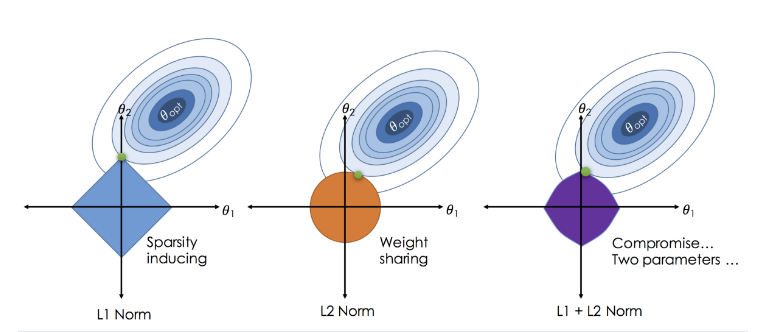
\includegraphics[width=\linewidth]{images/l1-l2-reg.png}
    \caption{一阶、二阶正则化效果示意图}
    \label{fig:l1-l2-reg}
\end{figure*}